% Datei: Documents/latex/minimalbeispiele/includegraphics/main.tex
% Begonnen: 13.02.2016 
% Letzte Änderung: 13.02.2016 
%
% Minimalbeispiel und Testumgebung für includegraphics
% Minimalbeispiel, weil mir in einigen Projekten plötzlich die Bilder abhanden gekommen sind.
% Der Grund war mir unklar. Durch Ausprobieren hat sich die Option 'dvipdfmx' als Ursache
% herausgestellt. Die habe ich vor längerer Zeit aktiviert, weil sie -- Quelle ist mir nicht mehr bekannt --
% eine lästige Fehlermeldung "cannot determne size of graphic" unterbunden hat.
% Die Bilder können mit dem graphicx-Package in der Präambel und comiliert mit PDFLatex wieder problemlos geladen werden.
% Des weiteren dient dieses Minimalbeispiel dem Testen der verschiedenen Optionen von includegraphics.

% parsip: Abstandsart (half: vertikaler Abstand halbe Zeile)
\documentclass[a4paper,parskip=half]{scrartcl}

\usepackage[utf8]{inputenc}
\usepackage[T1]{fontenc}
\usepackage[ngerman]{babel}

% Die Option dvipdfmx und das Paket bmpsize verhindern die Fehlermeldung von
% latex: "cannot determine size of graphic". Allerdings werden mit der Option
% dvipdfmx Bilder (getestet mit JPG) **überhaupt** nicht mehr angezeigt.
% \usepackage[dvipdfmx]{graphicx}
% \usepackage{bmpsize}

\usepackage[]{graphicx}

\begin{document}

\section*{Beipiel \texttt{includegraphics}}

% Positionsparameter: h:here, t:top, b:bottom, p:own page. Die Reihenfolge ist
% egal (?). Mit dem Ausrufezeichen (bang float) kann die Präferenz gesteuert
% werden und wird dann VOR das entsprechende Positionszeichen gesetzt.
\begin{figure}[!htb]
  \centering

  % Hängender Einzug ab der zweiten Zeile der Bildbeschreibung. Andere
  % Gestaltungsmöglichkeiten siehe KOMA-Script S. 159.
  \setcapindent{1em}
  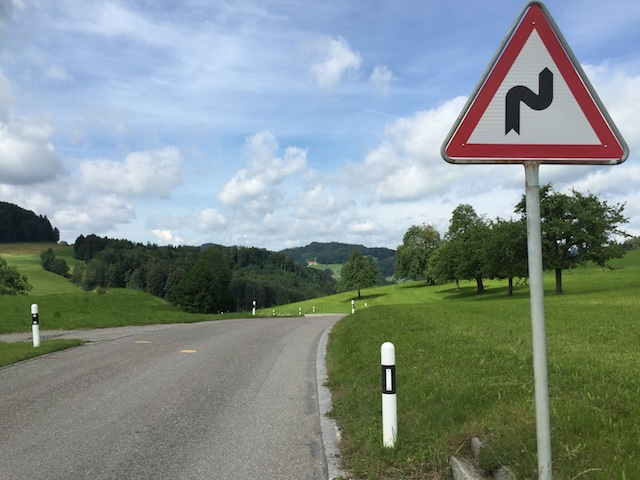
\includegraphics[%
    width=.8\textwidth,%
    angle=5,% dreht das Bild 5 Grad im GEGENUHRZEIGERSINN
    draft=FALSE,% bei TRUE wird nur eine Box und der Dateiname angezeigt
        ]{example.jpg}
    \caption[Lorem ipsum]{Lorem ipsum dolor sit amet, consectetuer adipiscing elit.
        Aenean commodo ligula eget dolor.
        Aenean massa. Cum sociis natoque penatibus et magnis dis parturient montes, nascetur ridiculus mus.
        Donec quam felis, ultricies nec, pellentesque eu, pretium quis, sem.
        Nulla consequat massa quis enim. Donec pede justo, fringilla vel, aliquet nec, vulputate.}
  \label{fig:example}
\end{figure}

\end{document}

